\begin{wrapfigure}[13]{r}{0.5\textwidth}
    \vspace{-0.1cm}
  \centering
    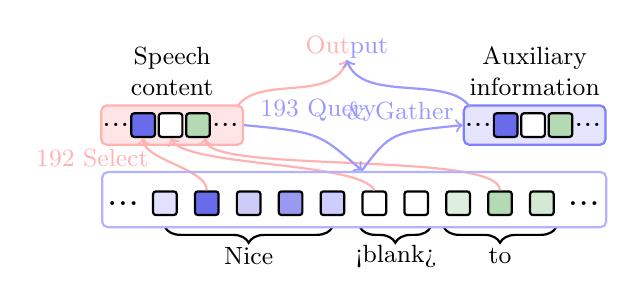
\begin{tikzpicture}[scale=0.92]
    \small{
      \node(c) at (0,0) 
      [rectangle, draw=black, fill={rgb,255:red,204; green,204; blue,255},  thick, minimum width=0.3cm,minimum height=0.3cm,rounded corners=1pt,align=center] {};
      \node(l2) at ([xshift=-0.4cm]c.west) 
      [rectangle, draw=black, fill={rgb,255:red,151; green,154; blue,240},  thick, minimum width=0.3cm,minimum height=0.3cm,rounded corners=1pt,align=center] {};  
      \node(l3) at ([xshift=-0.4cm]l2.west) 
      [rectangle, draw=black, fill={rgb,255:red,204; green,204; blue,248},  thick, minimum width=0.3cm,minimum height=0.3cm,rounded corners=1pt,align=center] {};  
      \node(l4) at ([xshift=-0.4cm]l3.west) 
      [rectangle, draw=black, fill={rgb,255:red,104; green,107; blue,234},  thick, minimum width=0.3cm,minimum height=0.3cm,rounded corners=1pt,align=center] {}; 
      \node(l5) at ([xshift=-0.4cm]l4.west) 
      [rectangle, draw=black, fill={rgb,255:red,224; green,224; blue,255},  thick, minimum width=0.3cm,minimum height=0.3cm,rounded corners=1pt,align=center] {}; 
      \node(r1) at ([xshift=0.4cm]c.east) 
      [rectangle, draw=black, fill={rgb,255:red,255; green,255; blue,255},  thick, minimum width=0.3cm,minimum height=0.3cm,rounded corners=1pt,align=center] {}; 
       \node(r2) at ([xshift=0.4cm]r1.east) 
      [rectangle, draw=black, fill={rgb,255:red,255; green,255; blue,255},  thick, minimum width=0.3cm,minimum height=0.3cm,rounded corners=1pt,align=center] {};
       \node(r3) at ([xshift=0.4cm]r2.east) 
      [rectangle, draw=black, fill={rgb,255:red,223; green,239; blue,223},  thick, minimum width=0.3cm,minimum height=0.3cm,rounded corners=1pt,align=center] {};
       \node(r4) at ([xshift=0.4cm]r3.east) 
      [rectangle, draw=black, fill={rgb,255:red,180; green,218; blue,180},  thick, minimum width=0.3cm,minimum height=0.3cm,rounded corners=1pt,align=center] {};
      \node(r5) at ([xshift=0.4cm]r4.east) 
      [rectangle, draw=black, fill={rgb,255:red,211; green,233; blue,211},  thick, minimum width=0.3cm,minimum height=0.3cm,rounded corners=1pt,align=center] {};
      \node(step1) at ([xshift=-0.1cm, yshift=0.45cm]l5.north) 
      [rectangle,  align=center,anchor=east] {{\color{red!30}\ding{192} Select}};
      \node() at([xshift=0.4cm]r5.east)  [rectangle, align=center] {\Large{...}};
      \node() at([xshift=-0.4cm]l5.west)  [rectangle, align=center] {\Large{...}};
      
      \node(q) at ([xshift=0.1cm,yshift=0.9cm]l5.north) [rectangle, draw=red!30, fill=red!10,  thick, minimum width=1.8cm,minimum height=0.5cm,rounded corners=2pt,align=center, anchor=center] {};
      \node(qt1) at (q.north) [rectangle, align=center, anchor=south] {Speech\\content};
      \node(qt2) at ([xshift=0.1cm,yshift=0.2cm]q.east) [rectangle, align=center, anchor=west] {{\color{blue!40}\ding{193} Query}};
      
      \node(q1) at ([xshift=-0.3cm,yshift=0.9cm]l5.north) 
      [rectangle, draw=black, fill={rgb,255:red,104; green,107; blue,234},  thick, minimum width=0.3cm,minimum height=0.3cm,rounded corners=1pt,align=center] {};
      \node(q2) at ([xshift=0.2cm]q1.east) 
      [rectangle, draw=black, fill=white,  thick, minimum width=0.3cm,minimum height=0.3cm,rounded corners=1pt,align=center,anchor=center] {};
      \node(q3) at ([xshift=0.2cm]q2.east) 
      [rectangle, draw=black, fill={rgb,255:red,180; green,218; blue,180},  thick, minimum width=0.3cm,minimum height=0.3cm,rounded corners=1pt,align=center,anchor=center] {};
      
      \node() at([xshift=-0.2cm]q1.west)  [rectangle, align=center] {\large{...}};
      \node() at([xshift=0.2cm]q3.east)  [rectangle, align=center] {\large{...}};

      \node(o) at ([xshift=-0.1cm,yshift=0.9cm]r5.north) [rectangle, draw=blue!50, fill=blue!10,  thick, minimum width=1.8cm,minimum height=0.5cm,rounded corners=2pt,align=center, anchor=center] {};
      \node(ot1) at (o.north) [rectangle, align=center, anchor=south] {Auxiliary\\information};
      \node(ot2) at ([yshift=0.2cm]o.west) [rectangle, align=center, anchor=east] {{\color{blue!40} \& Gather}};

      \node(o1) at ([xshift=-0.5cm,yshift=0.9cm]r5.north) 
      [rectangle, draw=black, fill={rgb,255:red,104; green,107; blue,234},  thick, minimum width=0.3cm,minimum height=0.3cm,rounded corners=1pt,align=center] {};
      \node(o2) at ([xshift=0.2cm]o1.east) 
      [rectangle, draw=black, fill=white,  thick, minimum width=0.3cm,minimum height=0.3cm,rounded corners=1pt,align=center,anchor=center] {};
      \node(o3) at ([xshift=0.2cm]o2.east) 
      [rectangle, draw=black, fill={rgb,255:red,180; green,218; blue,180},  thick, minimum width=0.3cm,minimum height=0.3cm,rounded corners=1pt,align=center,anchor=center] {};
      
      \node() at([xshift=-0.2cm]o1.west)  [rectangle, align=center] {\large{...}};
      \node() at([xshift=0.2cm]o3.east)  [rectangle, align=center] {\large{...}};

      \node(output) at ([xshift=0.2cm,yshift=1.7cm]c.north) [rectangle, align=center, anchor=south] {{\color{red!30}Out}{\color{blue!40}put}};

      \draw[decorate, decoration={brace,amplitude=2mm}, thick] ([yshift=-0.15cm]c.south) -- ([yshift=-0.15cm]l5.south);
      
      \draw[decorate, decoration={brace,amplitude=2mm}, thick] ([xshift=0.2cm, yshift=-0.15cm]r2.south) -- ([xshift=-0.2cm, yshift=-0.15cm]r1.south);

      \draw[decorate, decoration={brace,amplitude=2mm}, thick] ([xshift=0.2cm, yshift=-0.15cm]r5.south) -- ([xshift=-0.2cm, yshift=-0.15cm]r3.south);
      
      \node(nice) at ([yshift=-0.55cm]l3.south) [rectangle, align=center] {Nice};

      \node(blank) at ([xshift=0.3cm, yshift=-0.55cm]r1.south) [rectangle, align=center] {<blank>};
      \node(to) at ([yshift=-0.55cm]r4.south) [rectangle, align=center] {to};
      
      \draw[->,thick,color=red!30](l4.north).. controls ([yshift=0.3cm]l4.north) and ([yshift=-0.3cm]q1.south) ..(q1.south);
      \draw[->,thick,color=red!30](r1.north).. controls ([xshift=-0.2cm, yshift=0.4cm]r1.north) and ([xshift=0.2cm,yshift=-0.4cm]q2.south) ..(q2.south);
      \draw[->,thick,color=red!30](r4.north).. controls ([yshift=0.55cm]r4.north) and ([xshift=0.1cm,yshift=-0.5cm]q3.south) ..([xshift=0.1cm]q3.south);
      
      \draw[->,thick,color=blue!40](q.east).. controls ([yshift=-0.3cm]qt2.center)..([xshift=0.6cm,yshift=-0.55cm]qt2.south);
       %\draw[decorate, decoration={brace,amplitude=2.5mm}, thick,color=blue!20] ([xshift=-0.2cm, yshift=0.2cm]l5.west) -- ([xshift=0.2cm, yshift=0.2cm]r5.east);
       \node() at ([xshift=0.3cm,yshift=0.05cm]c) [rectangle, draw=blue!30, thick, minimum width=6.4cm,minimum height=0.7cm,rounded corners=2pt,align=center, anchor=center] {};
       \draw[->,thick,color=blue!40] ([xshift=0.6cm,yshift=-0.55cm]qt2.south).. controls ([xshift=1.0cm,yshift=-0.3cm]qt2.center).. (o.west);

       \draw[->,thick,color=red!30]([yshift=0.25cm,xshift=-0.1cm]q.east).. controls ([xshift=0.2cm,yshift=0.7cm]q.east) and ([xshift=-0.2cm,yshift=-0.5cm]output.south) ..([yshift=0.1cm]output.south);
       \draw[->,thick,color=blue!40]([yshift=0.25cm,xshift=0.1cm]o.west).. controls ([xshift=-0.2cm,yshift=0.7cm]o.west) and ([xshift=0.2cm,yshift=-0.5cm]output.south) ..([yshift=0.1cm]output.south);
      %\draw[->,thick](encoder.north)to([yshift=0.2cm]encoder.north)to([xshift=-0.2cm,yshift=0.7cm]decoder.west) to([xshift=-0.2cm]decoder.west)to(decoder.west);
      }
    \end{tikzpicture}
    
  
    \caption{We first select the features based on the peak of CTC prediction. Then, we use these features to query and gather auxiliary information from the original sequence. Finally, we fuse the two features to achieve shrinking. }
    \label{lbm_method}
    \vspace{-0.2cm}
\end{wrapfigure}